\documentclass[11pt]{article}
\usepackage[margin=0.75in]{geometry}
\usepackage{amsmath,amssymb,graphicx,hyperref}
\setlength{\parindent}{0pt}\setlength{\parskip}{4pt}
\setlength{\emergencystretch}{3em}
\begin{document}
{\Large Exact public kernel line and constrained rank repair}\par
2026-11-13. Source\path{4b6ed788d}. Unsigned evidence [pcc:unverified].

\textbf{Exact geometry.} Over a field, let $|S|=2a$, $a\ge2$, $\deg f=3$,
and $z(x)^2=f(x)$ on every actual node. Let $M$ be the public barycentric
Hankel matrix of size $a-1$. If $\det M=0$, then
\[
 \operatorname{rank}(M)+1=a-1,\qquad
 Mb=0\ \Longleftrightarrow\ \exists t\in K,\ b=t u
\]
for every nonzero actual kernel vector $u$. Numerical corank is derived,
not assumed. No successful $A/B$, primitive-polynomial premise, normalization,
square-root or rank oracle is supplied [pcc:unverified].

\textbf{Direct proof.} Actual reconstruction gives bounded $A_0,B_0,A_1,B_1$.
Shared node branches imply $G\mid A_0B_1-A_1B_0$, whose degree is below
$\deg G=2a$; hence the cross product is zero. The derived nonzero norm
identities then give $c_0B_1^2=c_1B_0^2$. Leading coefficients construct the
scalar ratio, and factoring a difference of squares yields $B_1=CtB_0$
without a root oracle. Injectivity of ofFn gives the vector line; ordinary
rank-nullity gives corank one. Zero vectors are handled separately
[pcc:unverified].

\begin{center}
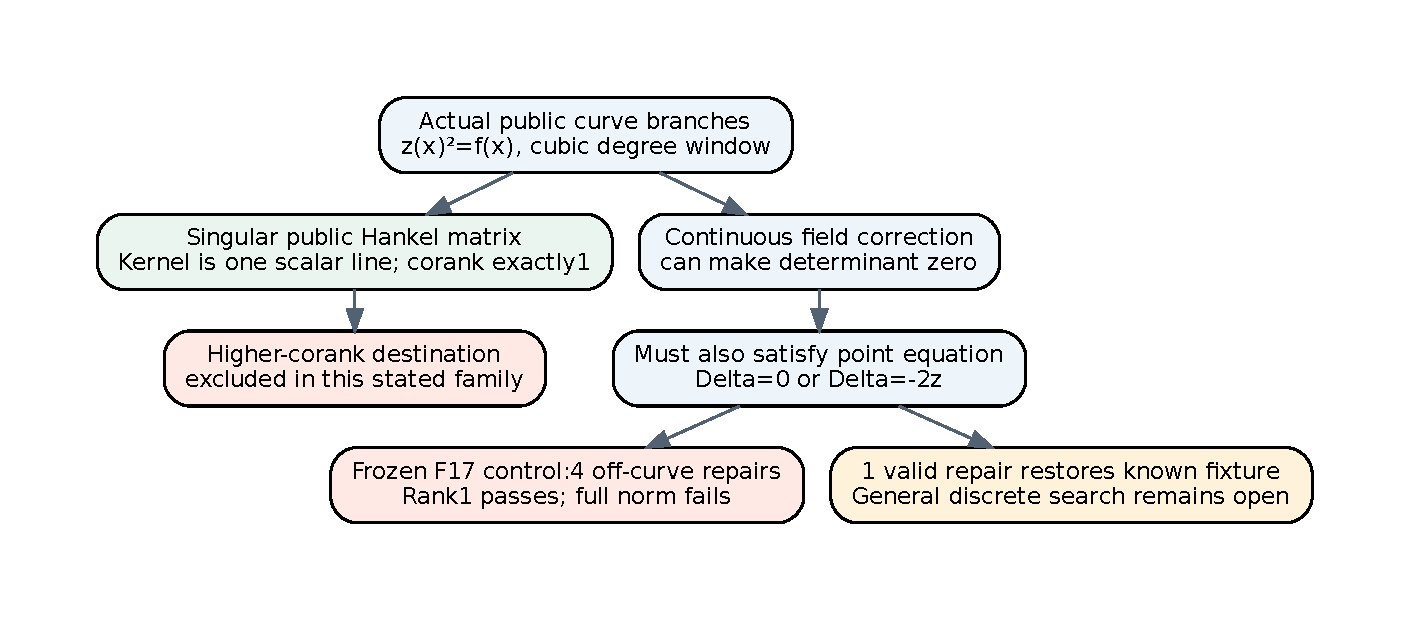
\includegraphics[width=0.94\linewidth,height=0.34\textheight,keepaspectratio]{repair.pdf}
\end{center}

\textbf{Curve constraint.} For every field,
\[
 (z+\Delta)^2=z^2\quad\Longleftrightarrow\quad
 \Delta=0\ \text{or}\ \Delta=-2z.
\]
Factor $\Delta(2z+\Delta)$. In characteristic2 the alternatives coincide;
for prime-curve inputs $p>3$, $z\ne0$, the only nontrivial correction is the
opposite branch. A field-valued determinant repair must satisfy this as well
as singularity [pcc:unverified].

A larger-corank target is excluded for this stated public family. This is
not a global ECDLP lower bound, a no-go result for all discrete searches,
or a map from the earlier $W$-jet proposal [pcc:unverified].

\newpage
{\Large Fixed repair controls and remaining search obligation}\par
Over F17 use $f=X^3+2X+2$ and supplied points
$(0,6),(3,1),(5,1),(6,3),(10,11),(13,10)$.
Initially $M=\left(\begin{smallmatrix}9&14\\14&3\end{smallmatrix}\right)$,
$\det M=1$. For $v=(1,x)$ set $h=w_x v^T\operatorname{adj}(M)v$.
If $h\ne0$, choose $\Delta=-\det M/h$ and rebuild the matrix. Record $h=0$
without dividing. All17 field corrections are tested for that frozen zero
direction [pcc:unverified].

\begin{center}\small
\begin{tabular}{rrrrl}
$x$ & $h$ & $\Delta$ & new $y$ & Actual curve / full norm\\\hline
0&12&7&13&fails / fails; target branch changes\\
3&0&--&--&no continuous repair in this direction\\
5&11&3&4&fails / fails\\
6&16&1&4&fails / fails\\
10&6&14&8&fails / fails\\
13&6&14&7&passes / passes
\end{tabular}
\end{center}
All five repaired matrices have determinant0 and rank1. Reconstruct every
kernel vector to $A/B$ and check repaired branch rows, degree bounds,
the actual curve equation and full norm.
The four off-curve repairs fail the full norm despite rank1. The one valid
repair restores the known positive fixture. These are fixed correctness cases,
not independent trials, a sign-search success rate or a runtime result
[pcc:unverified].

With target branch at $x=0$ fixed, only four repairs are eligible: three
fail the curve/norm and one passes; the same one zero direction remains.
These are two views of the same cases. A separate finite predicate check
covers all289 pairs $(z,\Delta)$ over F17 [pcc:unverified].

\textbf{Validation.} Eleven new statements in NormBranchRepair. Build001
fails on two interface details;002 passes and prints only standard Lean
foundations. Whole-study source audit and fresh import-inclusive replay have
exact receipts in checks.json/fresh-status.json. Eleven native tests,
strict clippy, release build001 and one write-once artifact invocation001
pass; failed source log/exit retained [pcc:unverified].

Kernel line: \path{PCC-20261113-98d020}.\par
Actual corank: \path{PCC-20261113-a3591d}.\par
Exact branch constraint: \path{PCC-20261113-59cebf}.\par
Original native artifact: \path{PCC-20261113-49efb0}.\par
All unsigned. Default-PATH source-only checks are not\_covered, separately
from explicit-toolchain kernel checks. Pinned Lean4.35.0, CryptoLean
\path{148f5dc389b}, Mathlib\path{cfc55fc58714}. The README contains the full
11-statement proof map, artifact hash and source-linked original evidence.

\textbf{Next action.} A candidate must implement genuinely discrete branch
selection or a different public factor-base construction with fewer counted
attempts, while keeping target, norm/divisor/scalar checks and total
$\exp(o(\log r))$ bit work. Continuous repair and higher corank do not supply
that result. No general existence/nonexistence theorem follows
[pcc:unverified].

\textbf{Sources.} Actual public Hankel construction and pinned polynomial/
rank-nullity declarations; previously opened Li--Wan--Zhang1501.01138
Proposition4.1 and Cheng cs/0507026 principal-divisor discussion. The proof is
direct algebra with no paper statement encoded as an axiom. KB unavailable:
MCP absent, wrapper has no executable. No novelty/exhaustive claim, paid run,
statistical yield or performance promotion.
\end{document}
